\documentclass[10pt]{article}
%% Specify the Express journal you are submitting to
%\usepackage[OME]{express}
\usepackage[OE]{express}

%\usepackage[BOE]{express}


\begin{document}

\title{Deep Brain Fluorescence Imaging with a Minimally Invasive Multimode Optical Fiber}

\author{Shay Ohayon\authormark{1,2,*},Antonio Caravaca-Aguirre\authormark{3}, Rafael Piestun\authormark{3}, James J. DiCarlo\authormark{1,2} }

\address{\authormark{1}McGovern Institute for Brain Research, Massachusetts Institute of Technology, 43 Vassar Street, Cambridge, MA 02139, USA\\
\authormark{2}Department of Brain and Cognitive Sciences, Massachusetts Institute of Technology, 77 Massachusetts Ave, Cambridge, MA 02139, USA\\
\authormark{3}Department of Electrical, Computer and Energy Engineering, University of Colorado, Boulder, Colorado 80309, USA}

\email{\authormark{*}shay.ohayon@gmail.com} %% email address is required

%%%%%%%%%%%%%%%%%%% abstract and OCIS codes %%%%%%%%%%%%%%%%

\begin{abstract}
A major open challenge in Neuroscience is the ability to
measure and perturb neural activity in vivo from well defined
neural sub-populations at cellular resolution
anywhere in the brain. However, limitations posed by
scattering and absorption prohibit non-invasive (surface)
multi-photon approaches for deep (>2mm) structures,
while Gradient Refractive Index (GRIN) endoscopes are
thick and cause significant damage upon insertion. Here, we
present a novel micro-endoscope design to image neural
activity at arbitrary depths via an ultra-thin multi-mode
optical fiber (MMF) probe that is 5-10X thinner than
commercially available micro-endoscopes. We demonstrate
micron-scale resolution, multi-spectral and volumetric
imaging. In contrast to previous approaches, we show
that this method has an improved acquisition speed that is
sufficient to capture rapid neuronal dynamics in-vivo in
rodents expressing a genetically encoded calcium indicator (GCaMP).
Our results emphasize the potential of this technology in
Neuroscience applications and open up possibilities for
cellular resolution imaging in previously unreachable brain
regions.
\end{abstract}

\ocis{(170.2520) Fluorescence Microscopy; (060.2350) Fiber optics imaging.} 

%%%%%%%%%%%%%%%%%%%%%%% References %%%%%%%%%%%%%%%%%%%%%%%%%
\bibliographystyle{osajnl}
\bibliography{references}
%%%%%%%%%%%%%%%%%%%%%%%%%%  body  %%%%%%%%%%%%%%%%%%%%%%%%%%
\section{Introduction}

Multi-photon surface based imaging techniques have been successfully applied in Neuroscience applications to image neurons and their activity at depths up to 1.6 mm relative to the cortical surface \cite{Horton2013-ce,Ouzounov2017-tg}. Many brain areas, however, lie beyond 1.6mm, especially in larger animals (e.g., ventral regions in non-human primates are 30mm deep relative to the dorsal surface).  The design requirements for deep imaging deep in NHPs can be different compared to deep imaging systems designed for rodents. For example, one may wish to image acutely and target regions based on functional properties (stimuli responses), or target multiple different populations in the same animal to increase throughput.  

To reach deeper, gradient refractive index lens (GRIN) based micro-endoscopes have been introduced \cite{Bocarsly2015-sa, Szabo2014-op,Mekhail2016-oi,Ghosh2011-mt}. However, GRIN lenses typically have a large diameter (0.5-1mm) and are difficult to fabricate at smaller diameters at long lengths due to their fragility. In addition, inserting such large diameter probes into the brain can cause significant damage and tissue displacement, which is why a common practice is to aspirate the brain above the region of interest to be imaged \cite{Barretto2012-kw}. 

To assess expected brain deformation induced by inserting probes of different diameters we ran experiments in which probes of varying diameter were inserted into gel with brain like consistency, sparsely filled with tiny platinum beads (figure \ref{fig:figure1}a). We imaged these phantom with stereo x-ray and registered beads position before and after probe insertion to assess the amount of tissue displacement and compression. We found that 1mm diameter probes induced large displacement (2.55 $\pm$ 1.93 mm) and compression (3.5mm shift of upper surface), while smaller diameter probes (0.1mm) induced shifts that were barely noticeable, suggesting the latter are better suited for acute-type experiments.  


\begin{figure}[ht!]
\centering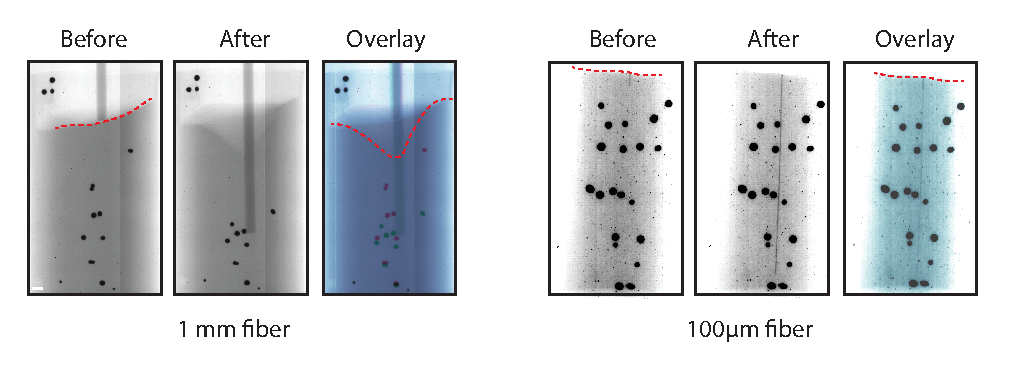
\includegraphics[width=15cm]{figure1}
\caption{\textbf{Simulations of expected brain tissue movement and compression}. Small platinum beads (0.1-1mm in diameter) were embedded in agarose gel with brain like consistency and imaged with stereo x-ray system (only one view of the stereo pair is shown). Comparison between  insertion of 1mm and 0.1mm probes. Dashed red lines denote surface deformation and false color image overlay shows beads movement (red - before insertion, blue - after insertion). }
\label{fig:figure1}
\end{figure}



Here, we present a new lens-less micro-endoscope (Fiberscope) that uses an ultra-thin (120$\mu m$) multi-mode optical fiber (MMF) to achieve micron-scale resolution imaging in-vivo. MMF have been previously used in in-vivo Neuroscience applications to deliver light for perturbing brain activity using Optogenetics  (e.g., \cite{Ohayon2013-bh}) and as single-pixel fluorescent imaging device (i.e., fiber-photometry \cite{Kim2016-ut,Gunaydin2014-ns}), but not for transmitting images since a speckle pattern is formed on the distal side when coherent light is focused on the proximal side \cite{Goodman2010-qm}. Recent advances in wave front shaping (WFS) theory, however, suggest that if the input-output transformation of the fiber can be measured, arbitrary light patterns can be formed on the distal side of the fiber by aligning phases and generating constructive interference only at the desired location\cite{Vellekoop2010-sz,Popoff2010-um,Psaltis2013-ov,Cizmar2011-cn,Cizmar2012-ha}. We sought to exploit these ideas for in-vivo functional calcium imaging by systematically addressing the open technical challenges.


\section{System Overview}  \label{system_overview}

We use wave-front shaping to modulate the light hitting the proximal side of the fiber such that when it exits the distal side it generates a micron-scale spot at a desired location (figure \ref{fig:figure3}). Fluorescent proteins in the sample are excited by the generated excitation spot and emit light that is collected by the same fiber. Emissions are measured with a sensitive photo-multiplier tube (PMT) on the distal side of the fiber.
Images are obtained by raster scanning spots (figure \ref{fig:figure3} Each spot corresponds to a different phase modulation pattern that is presented on the proximal side of the fiber (random access scanning is also possible). To address the challenging temporal requirements for real-time in-vivo full field  image acquisition we adopt an approach proposed by \cite{Conkey2012-qe}, where phase modulation is generated on an amplitude-only modulation device (digital mirror device, DMD).

\begin{figure}
\centering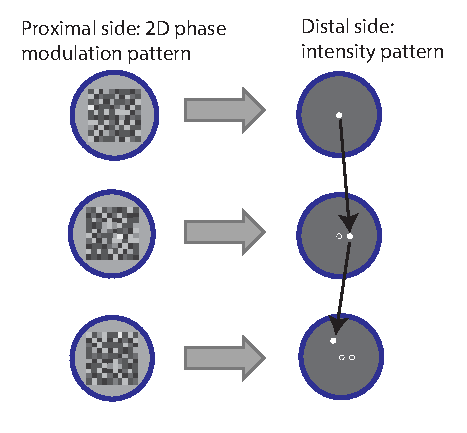
\includegraphics[width=8cm]{figure3}
\caption{\textbf{Fiber raster scanning}.}
\label{fig:figure3}
\end{figure}

The optical path of the micro-endoscope is presented in figure \ref{fig:figure2}. Overall, the system can be decomposed into four separate modules: 
\begin{enumerate}
\item Light generation module. This module has one output: the combined light from two DPSS lasers (473nm, laser quantum and 532nm, CNI laser). Light is combined with a dichroic beamsplitter (FF495-Di03-25x36, Semrock) into a SMF (single-mode fiber, SM400 from Thorlabs) using a fiber collimator (F220FC-532, Thorlabs). Two wave-lengths are not necessary for this technique, but do allow multi-spectral imaging (see section \ref{multi_spectral}).
\item  Light modulation module. This module has one input (SMF fiber from the light generation module) and two outputs: ultra-thin fiber that goes into the brain (100$\mu m$ core,120$\mu m$ total diameter, 0.66 NA from NeuroNexus) and a large diameter fiber (FG910UEC 910$\mu m$ 0.22 NA, Thorlabs) to carry emissions to the light collection module. The incoming light is expanded onto the surface of a DMD (V7000, Vialux) and relayed through a pin hole (1000$\mu m$, P1000 from Thorlabs) that blocks all but the first diffraction order. The light is passed through a multi-band dichroic filter (LF405/488/532/635-A-000, Semrock) and focused using a 40X objective (RMS40X, Thorlabs) on the thin imaging fiber. 
\item Light Collection module: this module receives the large diameter MMF fiber with fluorescence emissions, splits it into two bands using a dichroic beamsplitter (Di02-R561-25x36, Semrock) and measures emissions with PMTs (Thorlabs PMTSS and Hamamatsu H7422-40). The analog signal is amplified, filtered (SR570, Standford Research Systems) and digitized using a high speed DAQ (USB2020, 8MS/s, Measurement computing).
\item Calibration module: this module acquires images of the distal side of the fiber using a 10X objective (RMS10, Thorlabs) and a fast CMOS camera (MQ013MG-ON from Ximea, up to 1800 fps).

\end{enumerate}

The advantage of such modular design are clear. First, it enables mechanical motion of the imaging fiber without affecting the way light is coupled to the fiber (i.e., it will have no affect on the transmission matrix). Second, it reduces the weight of the module that needs to be mounted on a vertical translational stage. 

\begin{figure}[ht!]
\centering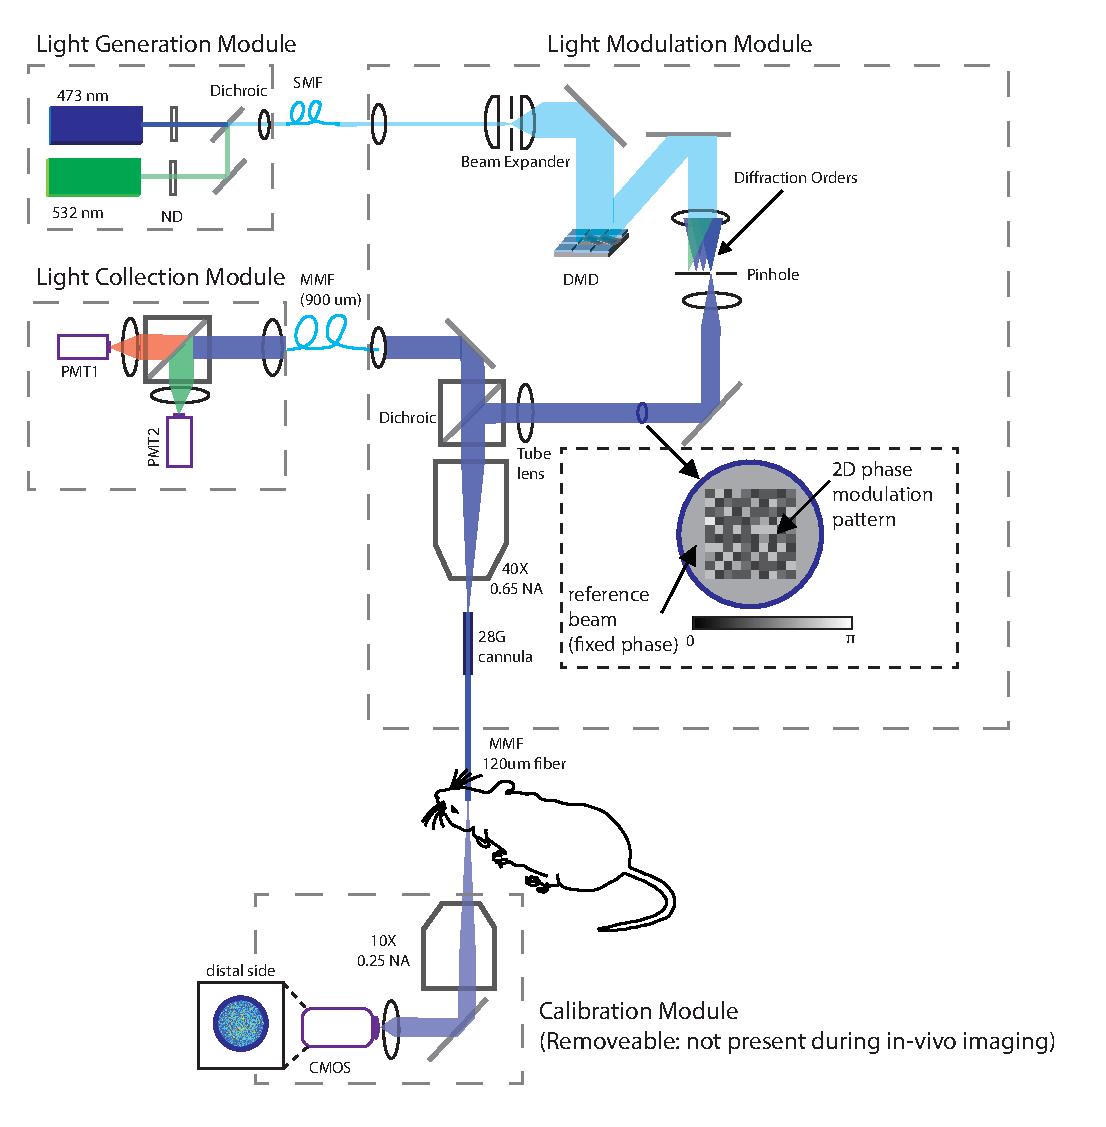
\includegraphics[width=15cm]{figure2}
\caption{\textbf{Optical system design}. See section \ref{optical_design} for details.}
\label{fig:figure2}
\end{figure}



\subsection{Phase modulation with a digital mirror device}
The basic concept that allows to generate phase modulation with amplitude-only modulation device is to create a special diffraction pattern that will have the desired spatial phase mask. The concept was first proposed by Lee \cite{Lee1978-ga}, and recently adopted on a digital mirror devices (DMD) by \cite{Conkey2012-qe}. Here, we make slight modifications to \cite{Conkey2012-qe} and propose to embed the desired spatial phase mask on a carrier function that is controlled by frequency $f$ and rotation $\theta$. Let $x$ and $y$ be the coordinates of a mirror on the DMD, then we define the carrier wave by:

% MathType!MTEF!2!1!+-
% feaagKart1ev2aaatCvAUfeBSjuyZL2yd9gzLbvyNv2CaerbuLwBLn
% hiov2DGi1BTfMBaeXatLxBI9gBaerbd9wDYLwzYbItLDharqqtubsr
% 4rNCHbGeaGqiVu0Je9sqqrpepC0xbbL8F4rqqrFfpeea0xe9Lq-Jc9
% vqaqpepm0xbba9pwe9Q8fs0-yqaqpepae9pg0FirpepeKkFr0xfr-x
% fr-xb9adbaqaaeGaciGaaiaabeqaamaabaabaaGcbaGaam4qamaabm
% aabaGaamiEaiaacYcacaWG5baacaGLOaGaayzkaaGaeyypa0Jaci4y
% aiaac+gacaGGZbWaaeWaaeaacqaH4oqCaiaawIcacaGLPaaacaWG4b
% Gaey4kaSIaci4CaiaacMgacaGGUbWaaeWaaeaacqaH4oqCaiaawIca
% caGLPaaacaWG5baaaa!4AFE!
\[C\left( {x,y} \right) = \cos \left( \theta  \right)x + \sin \left( \theta  \right)y\]

The continuously valued mask function: 

% MathType!MTEF!2!1!+-
% feaagKart1ev2aaatCvAUfeBSjuyZL2yd9gzLbvyNv2CaerbuLwBLn
% hiov2DGi1BTfMBaeXatLxBI9gBaerbd9wDYLwzYbItLDharqqtubsr
% 4rNCHbGeaGqiVu0Je9sqqrpepC0xbbL8F4rqqrFfpeea0xe9Lq-Jc9
% vqaqpepm0xbba9pwe9Q8fs0-yqaqpepae9pg0FirpepeKkFr0xfr-x
% fr-xb9adbaqaaeGaciGaaiaabeqaamaabaabaaGcbaGaamytamaabm
% aabaGaamiEaiaacYcacaWG5baacaGLOaGaayzkaaGaeyypa0ZaaSaa
% aeaacaaIXaaabaGaaGOmaaaadaqadaqaaiaaigdacqGHRaWkciGGJb
% Gaai4BaiaacohadaqadaqaaiaaikdacqaHapaCcaWGMbGaam4qamaa
% bmaabaGaamiEaiaacYcacaWG5baacaGLOaGaayzkaaGaeyOeI0Iaeu
% OPdy0aaeWaaeaacaWG4bGaaiilaiaadMhaaiaawIcacaGLPaaaaiaa
% wIcacaGLPaaaaiaawIcacaGLPaaaaaa!5406!
\[M\left( {x,y} \right) = \frac{1}{2}\left( {1 + \cos \left( {2\pi fC\left( {x,y} \right) - \Phi \left( {x,y} \right)} \right)} \right)\]

is then thresholded ($>0.5$) to decide which mirrors are turned on and off.
When this pattern is presented on the DMD, three main diffraction orders will be generated at the Fourier plane (0, $\pm1$). If only one of those is allowed to pass through a pinhole, the result will be a spatially modulated phase that is up to a fixed offset from the desired $\Phi \left( {x,y} \right)$. In the limit, each phase $\Phi \left( {x,y} \right)$ cannot be represented by a single mirror on the DMD, hence multiple mirrors are grouped to represent a single desired phase. 

\subsection{Transmission Matrix and Distal Side Pattern Generation}
We employ the Transmission Matrix method for measuring how input modes are scrambled to generate the observed speckle pattern. The full derivation of Transmission Matrix can be found in \cite{Popoff2010-um}. Here we give a brief summary. 
Under a linear model, we assume that the complex observed output $E^{out}$ linearly depends on the input modes: 

% MathType!MTEF!2!1!+-
% feaagKart1ev2aaatCvAUfeBSjuyZL2yd9gzLbvyNv2CaerbuLwBLn
% hiov2DGi1BTfMBaeXatLxBI9gBaerbd9wDYLwzYbItLDharqqtubsr
% 4rNCHbGeaGqiVu0Je9sqqrpepC0xbbL8F4rqqrFfpeea0xe9Lq-Jc9
% vqaqpepm0xbba9pwe9Q8fs0-yqaqpepae9pg0FirpepeKkFr0xfr-x
% fr-xb9adbaqaaeGaciGaaiaabeqaamaabaabaaGcbaGaamyramaaCa
% aaleqabaGaam4BaiaadwhacaWG0baaaOGaeyypa0Jaam4saiaacQca
% caWGfbWaaWbaaSqabeaacaWGPbGaamOBaaaaaaa!3F3A!
\[{E^{out}} = K*{E^{in}}\]

where $*$ denotes matrix multiplication and $K$ is the so called transmission matrix. The input field $E^{in}$ is a 2D complex field that is controlled by the phase mask:

% MathType!MTEF!2!1!+-
% feaagKart1ev2aaatCvAUfeBSjuyZL2yd9gzLbvyNv2CaerbuLwBLn
% hiov2DGi1BTfMBaeXatLxBI9gBaerbd9wDYLwzYbItLDharqqtubsr
% 4rNCHbGeaGqiVu0Je9sqqrpepC0xbbL8F4rqqrFfpeea0xe9Lq-Jc9
% vqaqpepm0xbba9pwe9Q8fs0-yqaqpepae9pg0FirpepeKkFr0xfr-x
% fr-xb9adbaqaaeGaciGaaiaabeqaamaabaabaaGcbaGaamyramaaCa
% aaleqabaGaamyAaiaad6gaaaGcdaqadaqaaiaadIhacaGGSaGaamyE
% aaGaayjkaiaawMcaaiabg2da9iaadgeacaWGLbWaaWbaaSqabeaacq
% aHapaCcaWGQbGaeuOPdy0aaeWaaeaacaWG4bGaaiilaiaadMhaaiaa
% wIcacaGLPaaaaaaaaa!4849!
\[{E^{in}}\left( {x,y} \right) = {e^{\pi j\Phi \left( {x,y} \right)}}\]

In the above derivation, $E^{in}$ is flattened to form a $Nx1$ vector, where $N$ is the number of independent modes that can be controlled (
in our case, N=4096, i.e. 64x64 modes). The complex output dimension equals the number of observed pixels on the distal side (roughly $\sim$10K).

If the calibration (mixing) matrix $K$ is known, any desired pattern can by synthesized by inverting the equation: 

% MathType!MTEF!2!1!+-
% feaagKart1ev2aaatCvAUfeBSjuyZL2yd9gzLbvyNv2CaerbuLwBLn
% hiov2DGi1BTfMBaeXatLxBI9gBaerbd9wDYLwzYbItLDharqqtubsr
% 4rNCHbGeaGqiVu0Je9sqqrpepC0xbbL8F4rqqrFfpeea0xe9Lq-Jc9
% vqaqpepm0xbba9pwe9Q8fs0-yqaqpepae9pg0FirpepeKkFr0xfr-x
% fr-xb9adbaqaaeGaciGaaiaabeqaamaabaabaaGcbaGaamyramaaCa
% aaleqabaGaaeyAaiaab6gacaqGFbGaae4yaiaabggacaqGSbGaae4y
% aaaakiabg2da9iaadUeadaahaaWcbeqaaiabgkHiTiaaigdaaaGcca
% WGfbWaaWbaaSqabeaacaqGKbGaaeyzaiaabohacaqGPbGaaeOCaiaa
% bwgacaqGKbaaaaaa!4876!
\[{E^{{\rm{in\_calc}}}} = {K^{ - 1}}{E^{{\rm{desired}}}}\]

Note that in practice, we can only synthesize phase modulation, so the actual pattern that is generated are the calculated phases of  $E^{in\_calc}$.

To measure $K$, one can present a large basis set of inputs:
% MathType!MTEF!2!1!+-
% feaagKart1ev2aaatCvAUfeBSjuyZL2yd9gzLbvyNv2CaerbuLwBLn
% hiov2DGi1BTfMBaeXatLxBI9gBaerbd9wDYLwzYbItLDharqqtubsr
% 4rNCHbGeaGqiVu0Je9sqqrpepC0xbbL8F4rqqrFfpeea0xe9Lq-Jc9
% vqaqpepm0xbba9pwe9Q8fs0-yqaqpepae9pg0FirpepeKkFr0xfr-x
% fr-xb9adbaqaaeGaciGaaiaabeqaamaabaabaaGcbaGaam4saiabg2
% da9iaadweadaahaaWcbeqaaiaab+gacaqGIbGaae4CaiaabwgacaqG
% YbGaaeODaiaabwgacaqGKbaaaOGaaiOkaiaadweadaahaaWcbeqaai
% aabkgacaqGHbGaae4CaiaabMgacaqGZbaaaaaa!4685!
\[K = {E^{{\rm{observed}}}}*{E^{{\rm{basis}}}}\]

where $E^{\rm{observed}}$ are the measured complex fields that correspond to the set of  complex input fields $E^{\rm{basis}}$. In our case, since 4096 input phases are controlled, $dim( E^{{\rm{basis}}}) = 4096x4096$.

We experimented with a number of different basis functions, including random, Hadamard and a polar version of the Hadamard version. All gave similar performance, so we ended up using the simple Hadamard which has the desired property $H^T = H^{-1}$:

% MathType!MTEF!2!1!+-
% feaagKart1ev2aaatCvAUfeBSjuyZL2yd9gzLbvyNv2CaerbuLwBLn
% hiov2DGi1BTfMBaeXatLxBI9gBaerbd9wDYLwzYbItLDharqqtubsr
% 4rNCHbGeaGqiVu0Je9sqqrpepC0xbbL8F4rqqrFfpeea0xe9Lq-Jc9
% vqaqpepm0xbba9pwe9Q8fs0-yqaqpepae9pg0FirpepeKkFr0xfr-x
% fr-xb9adbaqaaeGaciGaaiaabeqaamaabaabaaGcbaGaamyramaaCa
% aaleqabaGaaeOyaiaabggacaqGZbGaaeyAaiaabohaaaGcdaqadaqa
% aiaadIhacaGGSaGaamyEaiaacYcacaWGPbaacaGLOaGaayzkaaGaey
% ypa0JaamyzamaaCaaaleqabaGaeqiWdaNaamOAaiaadIeacaGGOaGa
% amiEaiaacYcacaWG5bGaaiilaiaadMgacaGGPaaaaaaa!4CA2!
\[{E^{{\rm{basis}}}}\left( {x,y,i} \right) = {e^{\pi jH(x,y,i)}}\],

where $H(x,y,i)$ represents the $i'th$ column in a 2D binary Hadamard matrix (i.e., reshaped from 4096x4096 to 64x64x4096).

To recover the complex output $E^{observed}$ we use an interferometric method proposed by \cite{Popoff2010-um}. The input field is padded with a constant phase reference. The two fields (reference, and 64x64 input modes) go through interference in the fiber such that there is no need for a separate reference arm. 
If the input pattern is shifted by a fixed amount $\alpha$, then the observed intensity will vary according to the following equation:

% MathType!MTEF!2!1!+-
% feaagKart1ev2aaatCvAUfeBSjuyZL2yd9gzLbvyNv2CaerbuLwBLn
% hiov2DGi1BTfMBaeXatLxBI9gBaerbd9wDYLwzYbItLDharqqtubsr
% 4rNCHbGeaGqiVu0Je9sqqrpepC0xbbL8F4rqqrFfpeea0xe9Lq-Jc9
% vqaqpepm0xbba9pwe9Q8fs0-yqaqpepae9pg0FirpepeKkFr0xfr-x
% fr-xb9adbaqaaeGaciGaaiaabeqaamaabaabaaGcbaGaamysamaaCa
% aaleqabaGaeqySdegaaOGaeyypa0ZaaqWaaeaacaWGfbWaaWbaaSqa
% beaacaWGVbGaamyDaiaadshaaaaakiaawEa7caGLiWoadaahaaWcbe
% qaaiaaikdaaaGccqGH9aqpdaabdaqaaiaadkhacqGHRaWkcaWGLbWa
% aWbaaSqabeaacaWGQbGaeqySdegaaOGaam4saiaacQcacaWGfbaaca
% GLhWUaayjcSdGaeyypa0ZaaqWaaeaacaWGYbaacaGLhWUaayjcSdWa
% aWbaaSqabeaacaaIYaaaaOGaey4kaSYaaqWaaeaacaWGlbGaaiOkai
% aadweaaiaawEa7caGLiWoadaahaaWcbeqaaiaaikdaaaGccqGHRaWk
% caaIYaGaaeOuaiaabwgadaqadaqaaiqadkhagaqeaiaadwgadaahaa
% WcbeqaaiaadQgacqaHXoqyaaGccaWGlbGaaiOkaiaadweaaiaawIca
% caGLPaaaaaa!66D0!
\[{I^\alpha } = {\left| {{E^{out}}} \right|^2} = \left| {r + {e^{j\alpha }}K*E} \right| = {\left| r \right|^2} + {\left| {K*E} \right|^2} + 2{\rm{Re}}\left( {\bar r{e^{j\alpha }}K*E} \right)\],

where $I^\alpha$ represents the measured power at a given pixel. If we define % MathType!MTEF!2!1!+-
% feaagKart1ev2aaatCvAUfeBSjuyZL2yd9gzLbvyNv2CaerbuLwBLn
% hiov2DGi1BTfMBaeXatLxBI9gBaerbd9wDYLwzYbItLDharqqtubsr
% 4rNCHbGeaGqiVu0Je9sqqrpepC0xbbL8F4rqqrFfpeea0xe9Lq-Jc9
% vqaqpepm0xbba9pwe9Q8fs0-yqaqpepae9pg0FirpepeKkFr0xfr-x
% fr-xb9adbaqaaeGaciGaaiaabeqaamaabaabaaGcbaGaamiuaiablY
% LiajqadkhagaqeaiaadUeacaGGQaGaamyraaaa!3B71!
$P \buildrel \Delta \over = \bar rK*E$
and 
% MathType!MTEF!2!1!+-
% feaagKart1ev2aaatCvAUfeBSjuyZL2yd9gzLbvyNv2CaerbuLwBLn
% hiov2DGi1BTfMBaeXatLxBI9gBaerbd9wDYLwzYbItLDharqqtubsr
% 4rNCHbGeaGqiVu0Je9sqqrpepC0xbbL8F4rqqrFfpeea0xe9Lq-Jc9
% vqaqpepm0xbba9pwe9Q8fs0-yqaqpepae9pg0FirpepeKkFr0xfr-x
% fr-xb9adbaqaaeGaciGaaiaabeqaamaabaabaaGcbaGaamyuaiablY
% LianaalaaabaGaaGymaaqaaiaaikdaaaWaamWaaeaacaWGjbWaaWba
% aSqabeaacaaIWaaaaOGaeyOeI0IaamysamaaCaaaleqabaGaeqiWda
% Naai4laiaaikdaaaGccqGHRaWkcaWGQbWaaeWaaeaacaWGjbWaaWba
% aSqabeaacqaHapaCcaGGVaGaaGOmaaaakiabgkHiTiaadMeadaahaa
% Wcbeqaaiabec8aWbaaaOGaayjkaiaawMcaaaGaay5waiaaw2faaaaa
% !4DAB!
$Q \buildrel \Delta \over = \frac{1}{2}\left[ {{I^0} - {I^{\pi /2}} + j\left( {{I^{\pi /2}} - {I^\pi }} \right)} \right]$,
we can recover the complex value $P$ since:
% MathType!MTEF!2!1!+-
% feaagKart1ev2aaatCvAUfeBSjuyZL2yd9gzLbvyNv2CaerbuLwBLn
% hiov2DGi1BTfMBaeXatLxBI9gBaerbd9wDYLwzYbItLDharqqtubsr
% 4rNCHbGeaGqiVu0Je9sqqrpepC0xbbL8F4rqqrFfpeea0xe9Lq-Jc9
% vqaqpepm0xbba9pwe9Q8fs0-yqaqpepae9pg0FirpepeKkFr0xfr-x
% fr-xb9adbaqaaeGaciGaaiaabeqaamaabaabaaGcbaGaamyuaiabg2
% da9maadmaabaGaaeOuaiaabwgadaqadaqaaiaadcfaaiaawIcacaGL
% PaaacqGHsislcaqGsbGaaeyzamaabmaabaGaamOAaiaadcfaaiaawI
% cacaGLPaaacqGHRaWkcaWGQbWaaeWaaeaacaqGsbGaaeyzamaabmaa
% baGaam4AaiaadcfaaiaawIcacaGLPaaacqGHsislcaqGsbGaaeyzam
% aabmaabaGaeyOeI0IaamiuaaGaayjkaiaawMcaaaGaayjkaiaawMca
% aaGaay5waiaaw2faaaaa!5230!
\[Q = \left[ {{\rm{Re}}\left( P \right) - {\rm{Re}}\left( {jP} \right) + j\left( {{\rm{Re}}\left( {kP} \right) - {\rm{Re}}\left( { - P} \right)} \right)} \right]\]

and

% MathType!MTEF!2!1!+-
% feaagKart1ev2aaatCvAUfeBSjuyZL2yd9gzLbvyNv2CaerbuLwBLn
% hiov2DGi1BTfMBaeXatLxBI9gBaerbd9wDYLwzYbItLDharqqtubsr
% 4rNCHbGeaGqiVu0Je9sqqrpepC0xbbL8F4rqqrFfpeea0xe9Lq-Jc9
% vqaqpepm0xbba9pwe9Q8fs0-yqaqpepae9pg0FirpepeKkFr0xfr-x
% fr-xb9adbaqaaeGaciGaaiaabeqaamaabaabaaGcbaGaamiuaiabg2
% da9maalaaabaGaaGymaaqaaiaaikdaaaWaaeWaaeaacaqGsbGaaeyz
% amaabmaabaGaamyuaaGaayjkaiaawMcaaiabgUcaRiGacMeacaGGTb
% WaaeWaaeaacaWGrbaacaGLOaGaayzkaaaacaGLOaGaayzkaaGaey4k
% aSYaaSaaaeaacaaIXaaabaGaaGOmaaaacaWGQbWaaeWaaeaacaqGsb
% GaaeyzamaabmaabaGaamyuaaGaayjkaiaawMcaaiabgkHiTiGacMea
% caGGTbWaaeWaaeaacaWGrbaacaGLOaGaayzkaaaacaGLOaGaayzkaa
% aaaa!5207!
\[P = \frac{1}{2}\left( {{\rm{Re}}\left( Q \right) + {\mathop{\rm Im}\nolimits} \left( Q \right)} \right) + \frac{1}{2}j\left( {{\rm{Re}}\left( Q \right) - {\mathop{\rm Im}\nolimits} \left( Q \right)} \right)\]

 Notice that once we know $P$, we can recover $K$ up to a unknown scale:
 
\subsection{Mechanical Design} \label{mechanical_design}
To reduce manufacturing costs, we used off-the-shelf components and mounted the optics between two aluminum boards (figure \ref{fig:figure13}). The design essentially folds the beam to reduce the overall form factor. This imaging module was mounted on a vertical translational stage (LS300, Thorlabs) that allowed to translate the imaging fiber without affecting the way phases were coupled to the proximal side. All Solidworks design files are publicly available on \url{https://github.com/dicarlolab/Fiberscope}/

\begin{figure}[ht!]
\centering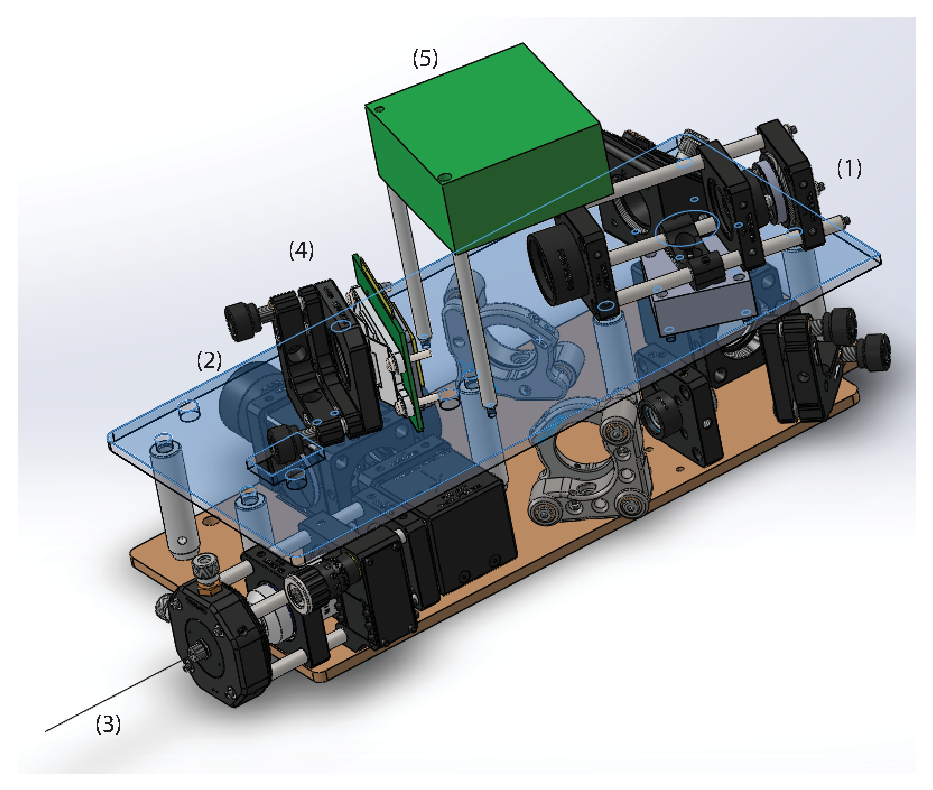
\includegraphics[width=15cm]{figure13}
\caption{\textbf{Mechanical system design}. See section \ref{mechanical_design} for details. Main components highlighted: (1) SMF entry port for a incoming light, (2) exit port for fluorescence emissions (large diameter MMF fiber), (3) thin (120$\mu m$) optical fiber used for imaging, (4) DMD, (5) DMD PCB controller. }
\label{fig:figure13}
\end{figure}

\subsection{Code Optimization}
To speed up calculations we wrote custom C++ code that uses Cublas (Cuda optimized matrix library for GPU). Further speed up was obtained by implementing a parallel Lee Hologram generator function on the GPU (10K holograms in less than 1.4 sec). Its output is represented as a packed binary image that can be uploaded faster to the DMD ($\sim$6.5 sec). All code is publicly available on \url{github: https://github.com/dicarlolab/Fiberscope}.

\section{Methods}
\subsection{Enhancement Factor Metric}\label{EnhancementFactor}
One of the key factors determining  SNR in our system is the peak intensity generated at the center of the point spread function. In previous studies (e.g. \cite{Conkey2012-qe}) SNR was quantified as the ratio between the peak and the average intensity of the background, a quantity termed the Enhancement Factor  (EF). 

The peak intensity can be several orders of magnitude brighter than the background and if both the peak and background are measured with a single exposure with a standard cameras that has a limited dynamic range, it can lead to strong bias and over-estimation of the EF.

To overcome this difficulty we devised a procedure in which multiple images of the fiber are taken under varying neutral density filters. All images are then merged back to form a single high dynamic range (HDR) image from which both peak and background can be reliably estimated without concerns of under or over exposed pixels. 

For a given image taken with neutral density $n$, a dark image is subtracted and all pixels that are over-exposed or under-exposed are
removed (we use 5\% and 95\% percentile values of the 12-bit camera range to define over and under exposures). The final HDR image is constructed using the remaining valid pixels using the following equation:

% MathType!MTEF!2!1!+-
% faaagCart1ev2aaaKnaaaaWenf2ys9wBH5garuavP1wzZbItLDhis9
% wBH5garmWu51MyVXgaruWqVvNCPvMCaebbnrfifHhDYfgasaacH8sr
% ps0lbbf9q8WrFfeuY-ribbf9v8qqaqFr0xc9pk0xbba9q8WqFfea0-
% yr0RYxir-Jbba9q8aq0-yq-He9q8qqQ8frFve9Fve9Ff0dc9Gqpi0d
% meaabaqaciGacaGaaeqabaWaaeaaeaaakeaacaqGibGaaeiraiaabk
% fadaqadaqaaiaadIhacaGGSaGaamyEaaGaayjkaiaawMcaaiabg2da
% 9maaxababaGaciyBaiaacggacaGG4baaleaacaWGUbaabeaakiaaig
% dacaaIWaWaaWbaaSqabeaacaWGUbaaaOWaaeWaaeaacaWGjbWaaeWa
% aeaacaWG4bGaaiilaiaadMhacaGGSaGaamOBaaGaayjkaiaawMcaai
% abgkHiTiaadMeadaWgaaWcbaGaamizaiaadggacaWGYbGaam4Aaaqa
% baGcdaqadaqaaiaadIhacaGGSaGaamyEaaGaayjkaiaawMcaaaGaay
% jkaiaawMcaaaaa!51D3!
\[{\rm{HDR}}\left( {x,y} \right) = \mathop {\max }\limits_n {10^n}\left( {I\left( {x,y,n} \right) - {I_{dark}}\left( {x,y} \right)} \right)\]

Finally, the enhancement factor is defined as $I_{peak} / I_{avg}$ where $I_{avg}$ is the average of the HDR image in the fiber core region after a 5x5 pixel region has been cropped around the $I_{peak}$'s location.

\subsection{Animal experiments}
All procedures have been approved by the Massachusetts Institute of Technology Institutional Animal Care and Use Committee and conform to NIH standards.
Wild type mice (C56BL) from Jackson Labs were anesthetized with isoflurane (1-2\%). A small borehole  ($\sim$300-500$\mu m$) was drilled and 50-100nl of AAV9-hSynGCaMP6s was pressure injected using a custom pump (25nl/minute) to deliver the GCaMP gene. We allowed 2-3 weeks of recovery and virus expression prior to imaging. Mice were then anesthetized again and a slightly larger
craniotomy was performed to expose the brain. We used a thin wall hypodermic needle (28G) as
reinforcement on the upper part of the fiber, leaving $\sim$2-5mm of fiber exposed for insertion (the needle was not pushed in the brain). Animals were then raised on a custom movable translational
stage in small increments until the fiber punctured through the dura and entered the brain. At the end of the imaging session, animals were euthanized with a lethal dose of pentobarbital. 

\section{Experimental Results}

\subsection{SNR and Enhancement Factor}
Following the procedure described in section \ref{EnhancementFactor}, we constructed a HDR image of the fiber after generating a spot at a single location (figure \ref{fig:figure4}a).
We then repeated this procedure and generated spots in all possible locations in the core by acquiring HDR image per spot location. We found that the distribution of EF values can vary significantly as a function of the coupling at the proximal side. Empirically, when more central modes were excited, a skewed EF distribution was observed and  central pixels had higher EF compared to pixels in the periphery (figure \ref{fig:figure4}b left). In contrast, after a slightly shift of the incident angle a obtain a more uniform distribution of EF across the core could be achieved, albeit with somewhat lower EF values (figure \ref{fig:figure4}b, right)

\begin{figure}
\centering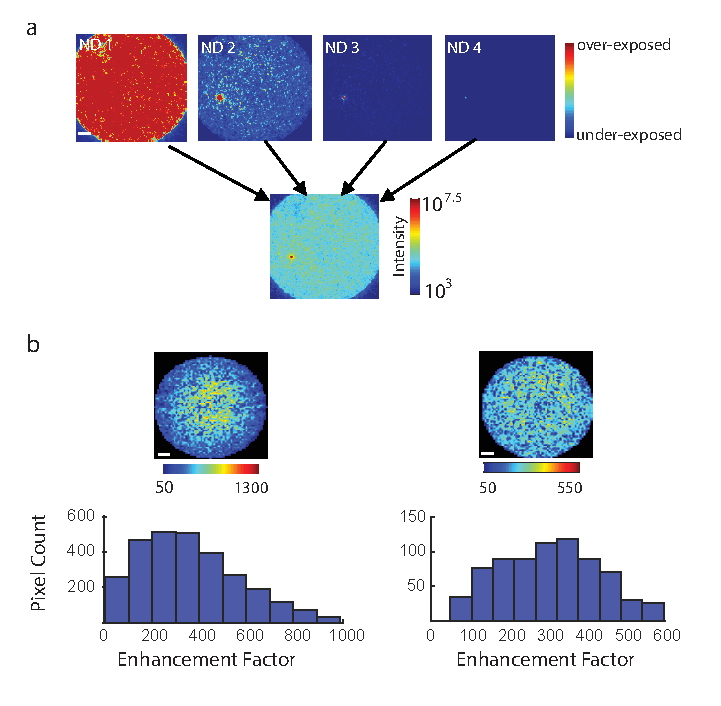
\includegraphics[width=13cm]{figure4}
\caption{\textbf{Enhancement Factor Estimation}. a) Images of the fiber taken under increasing levels of ND filters are combined to form HDR image. b) Two examples of observed distribution of enhancement factor values across the core.}
\label{fig:figure4}
\end{figure}

Another important factor determining the amplitude of the PSF is the number of input modes used and how many mirrors are assigned per input mode. Selecting these two parameters constrain the number of pixels that remain free to represent the constant reference arm. We experimented with 32x32, 64x64 and 96x96 modes and 8-12 mirrors per mode and found that the optimal combination with our DMD (V7000, Vialux, 1024x768 resolution) is 64x64 (4096 modes), where each mode is represented by 12 mirrors (figure \ref{fig:figure14}). Thus, the actual pattern that is modulated is 768x768, where the remainder 128x768 mirrors represent the reference beam.

\begin{figure}
\centering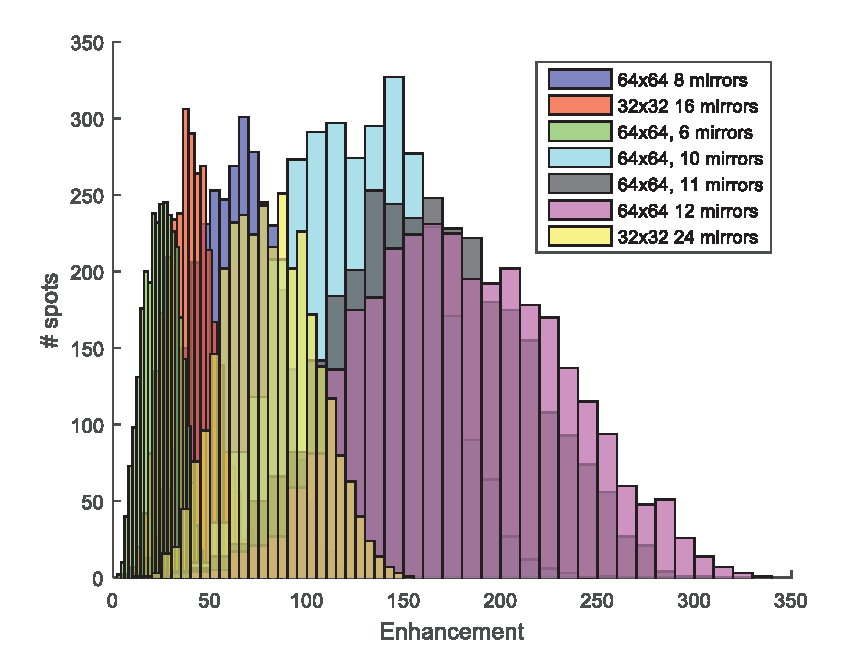
\includegraphics[width=10cm]{figure14}
\caption{\textbf{Reference and modes trade-off }. Enhancement factor distribution as a function of number of input modes and number of mirrors assigned per mode.}
\label{fig:figure14}
\end{figure}

\subsection{Point Spread Function}
To assess the optical quality we measured the point spread function (PSF)
along the emission path by imaging 0.96um fluorescent micro-spheres (figure \ref{fig:figure6}). We modeled the PSF as a 2D Gaussian

% MathType!MTEF!2!1!+-
% feaagKart1ev2aaatCvAUfeBSjuyZL2yd9gzLbvyNv2CaerbuLwBLn
% hiov2DGi1BTfMBaeXatLxBI9gBaerbd9wDYLwzYbItLDharqqtubsr
% 4rNCHbGeaGqiVu0Je9sqqrpepC0xbbL8F4rqqrFfpeea0xe9Lq-Jc9
% vqaqpepm0xbba9pwe9Q8fs0-yqaqpepae9pg0FirpepeKkFr0xfr-x
% fr-xb9adbaqaaeGaciGaaiaabeqaamaabaabaaGcbaGaamOramaabm
% aabaGaamiEaiaacYcacaWG5baacaGLOaGaayzkaaGaeyypa0Jaamyq
% aiaadwgadaahaaWcbeqaaiabgkHiTmaadmaabaWaaSaaaeaadaqada
% qaaiaadIhacqGHsislcaWG4bWaaSbaaWqaaiaaicdaaeqaaaWccaGL
% OaGaayzkaaWaaWbaaWqabeaacaaIYaaaaaWcbaGaaGOmaiabeo8aZn
% aaDaaameaacaWG4baabaGaaGOmaaaaaaWccqGHRaWkdaWcaaqaamaa
% bmaabaGaamyEaiabgkHiTiaadMhadaWgaaadbaGaaGimaaqabaaali
% aawIcacaGLPaaadaahaaadbeqaaiaaikdaaaaaleaacaaIYaGaeq4W
% dm3aa0baaWqaaiaadMhaaeaacaaIYaaaaaaaaSGaay5waiaaw2faaa
% aaaaa!574C!
\[F\left( {x,y} \right) = A{e^{ - \left[ {\frac{{{{\left( {x - {x_0}} \right)}^2}}}{{2\sigma _x^2}} + \frac{{{{\left( {y - {y_0}} \right)}^2}}}{{2\sigma _y^2}}} \right]}}\]

and fitted the data to the observed intensities. We found that the full width half maximum is 2.10$\pm$0.25 um (mean, std), with estimated SNR of 1.39$\pm$0.1.

\begin{figure}
\centering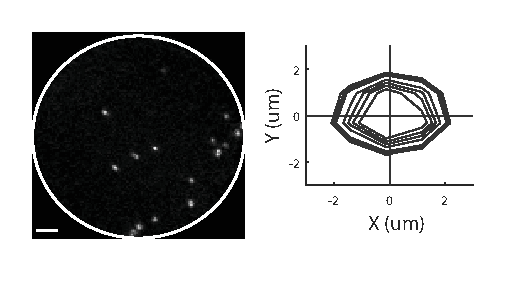
\includegraphics[width=12cm]{figure6}
\caption{\textbf{Point Spread Function}. The in plane resolution of the system was estimated by imaging 0.8$\mu m$ fluorescent beads and fitting 2D Gaussian to the data. The distribution of such fits are shown on the right.}
\label{fig:figure6}
\end{figure}



\subsection{Volumetric Imaging}\label{volumetric_imaging}
The ability to image away from the tip in the brain is important since neuron close to the tip are more likely to be damaged. When the calibration camera is focused on the fiber tip, the TM will map input phases to that plane. However, the imaging plane of the calibration camera can be translated downward. By doing this, the TM will still map input phases to the imaging plane and allow to form spots away from the fiber tip. Thus, It is possible to find phases needed to raster scan at different Z distances away from the tip, essentially acquiring a volume without the need to physically move the fiber during imaging (figure \ref{fig:figure5}a). 


To assess our ability to form excitation spots
away from the fiber tip in a scattering medium we imaged 15$\mu m$ micro-spheres embedded in 2\% intra-lipid agarose (figure \ref{fig:figure5}). To quantify how well we can form excitation spot in this scattering medium, we measured the separability of the bead relative to the background using the d' sensitivity index:


% MathType!MTEF!2!1!+-
% faaagCart1ev2aaaKnaaaaWenf2ys9wBH5garuavP1wzZbItLDhis9
% wBH5garmWu51MyVXgaruWqVvNCPvMCaebbnrfifHhDYfgasaacH8sr
% ps0lbbf9q8WrFfeuY-ribbf9v8qqaqFr0xc9pk0xbba9q8WqFfea0-
% yr0RYxir-Jbba9q8aq0-yq-He9q8qqQ8frFve9Fve9Ff0dc9Gqpi0d
% meaabaqaciGacaGaaeqabaWaaeaaeaaakeaacaWGKbGaai4jaiabg2
% da9maalaaabaGaeqiVd02aaSbaaSqaaiaadkeacaWGLbGaamyyaiaa
% dsgaaeqaaOGaeyOeI0IaeqiVd02aaSbaaSqaaiaadkeacaWGHbGaam
% 4yaiaadUgacaWGNbGaamOCaiaad+gacaWG1bGaamOBaiaadsgaaeqa
% aaGcbaWaaOaaaeaadaWcaaqaaiaaigdaaeaacaaIYaaaamaabmaaba
% Gaeq4Wdm3aa0baaSqaaiaadkeacaWGLbGaamyyaiaadsgaaeaacaaI
% YaaaaOGaey4kaSIaeq4Wdm3aa0baaSqaaiaadkeacaWGHbGaam4yai
% aadUgacaWGNbGaamOCaiaad+gacaWG1bGaamOBaiaadsgaaeaacaaI
% YaaaaaGccaGLOaGaayzkaaaaleqaaaaaaaa!5BCC!
\[d' = \frac{{{\mu _{Bead}} - {\mu _{Background}}}}{{\sqrt {\frac{1}{2}\left( {\sigma _{Bead}^2 + \sigma _{Background}^2} \right)} }}\]

We found that the separability index increased as the imaging plane got closer to 100 $\mu m$, suggesting the sharpest
focus was obtained at that Z-section (figure \ref{fig:figure5}b). 

\begin{figure}
\centering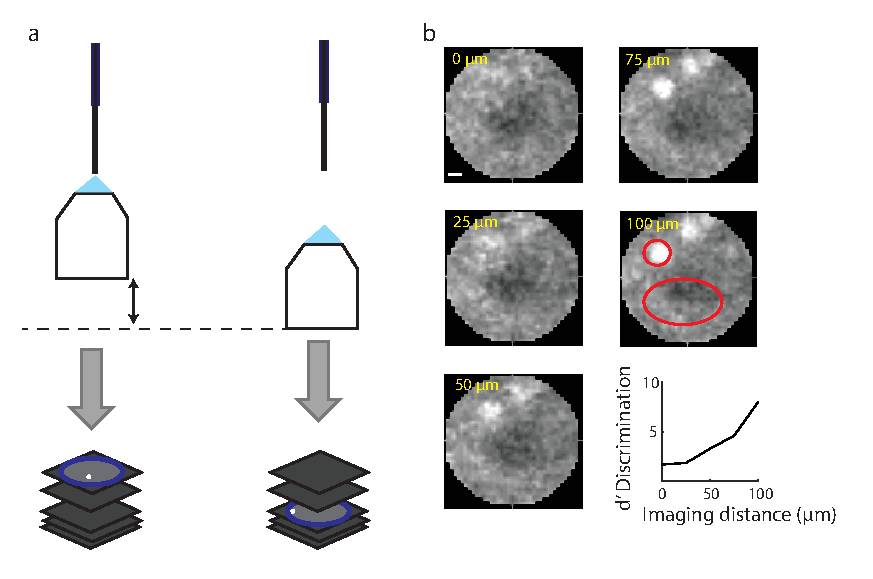
\includegraphics[width=10cm]{figure5}
\caption{\textbf{Volumetric Imaging}. a) Measuring transmission matrix (TM) with a camera focused on the tip can be used to generate spots on the tip. Measuring the TM with a camera that is focused at distance $z$ from the tip can be used to generate spots at distance $d$ from the fiber tip. b) Five sections of the same sample obtained at increasing distances from the fiber tip, collected without moving the fiber (i.e., with five different transmission matrices).  }
\label{fig:figure5}
\end{figure}

\subsection{Multi-Spectral Imaging}\label{multi_spectral}
In some Neuroscience applications it is desired to excite a subset of the field of view with one wavelength while monitoring the remainder with another wavelength. For example, one may wish to stimulate a given neuron with a red-shifted ChR2 variant \cite{Klapoetke2014-ea}, while monitoring the rest of the field of view using GCaMP. 

A nice advantage of using the pinhole for phase modulation in combination is that we can easily switch between two laser sources at the kHz range by adjusting the carrier wave function used to construct the hologram. 
The grating equation 
% MathType!MTEF!2!1!+-
% feaagKart1ev2aaatCvAUfeBSjuyZL2yd9gzLbvyNv2CaerbuLwBLn
% hiov2DGi1BTfMBaeXatLxBI9gBaerbd9wDYLwzYbItLDharqqtubsr
% 4rNCHbGeaGqiVu0Je9sqqrpepC0xbbL8F4rqqrFfpeea0xe9Lq-Jc9
% vqaqpepm0xbba9pwe9Q8fs0-yqaqpepae9pg0FirpepeKkFr0xfr-x
% fr-xb9adbaqaaeGaciGaaiaabeqaamaabaabaaGcbaGaamOBaiabeU
% 7aSjabg2da9iaadsgaciGGZbGaaiyAaiaac6gacqaHXoqycqGHRaWk
% ciGGZbGaaiyAaiaac6gacqaHYoGyaaa!445E!
$n\lambda  = d\sin \alpha  + \sin \beta $ shows that for a given incident angle $\alpha$, the $n$'th order reflection angle $\beta$ will depend on the wavelength $\lambda$. In our setup, with a reasonable incident angle ($\sim$40-65$\deg$), one can get $\sim$0.5$\deg$ difference in the reflected blue and green beams (both share the same incident angle), which maps to 1mm spatial difference for the first diffraction order at distances $>200mm$. By selecting the carrier wave frequency and rotation we can shift the position of the first diffraction order of one wave-length relative to the pinhole such that only that one will pass through (figure \ref{fig:figure7}a). Each wavelength requires its own calibration, but once obtained, it is possible to rapidly (22kHz) switch between the two sources and generate spots of different colors.
Our setup (figure \ref{fig:figure2}) also allows simultaneous acquisition of multi-spectral tissue using a single wave-length excitation. For example, figure \ref{fig:figure7}b shows an overlay of  two images obtained from the two PMTs when two different types of micro-spheres were mixed together (i.e., both excited by blue-wavelength but differ in their emission spectra).

\begin{figure}
\centering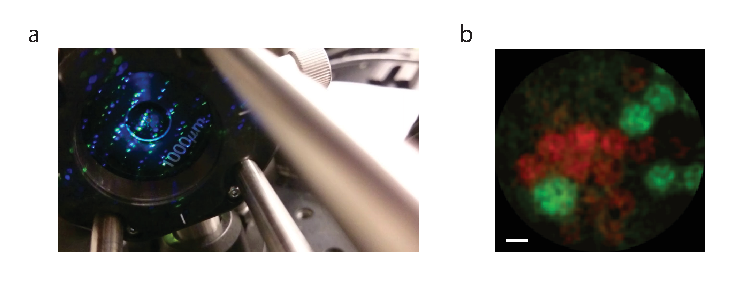
\includegraphics[width=12cm]{figure7}
\caption{\textbf{Multispectral imaging}. a) Rapid switching of the two excitation wavelengths is possible by steering the desired beam into the pinhole on the Fourier plane. This is achieved by changing the hologram carrier wave frequency and rotation.}
\label{fig:figure7}
\end{figure}

\subsection{Biological Tissue Imaging}\label{biological_imaging}
So far we demonstrated that our micro-endoscope can image fluorescent micro-spheres. However, biological fluorescence can be 10-1000 dimmer compared to such samples. To assess photon collection efficiency in more realistic conditions we imaged baby hamster kidney cells (BHK) expressing GFP. Our setup (figure \ref{fig:figure12}a) comprised of a sample on glass slice sandwiched between the micro-endoscope (top) and epi-fluorescence imaging microscope (bottom), where the latter represented "ground-truth" image. We found that BHK cells were sufficiently bright to be captured with our imaging system using a high NA fiber (figure \ref{fig:figure12}b) and that the acquired images had high correlation to the ground truth data (figure \ref{fig:figure12}c).


\begin{figure}
\centering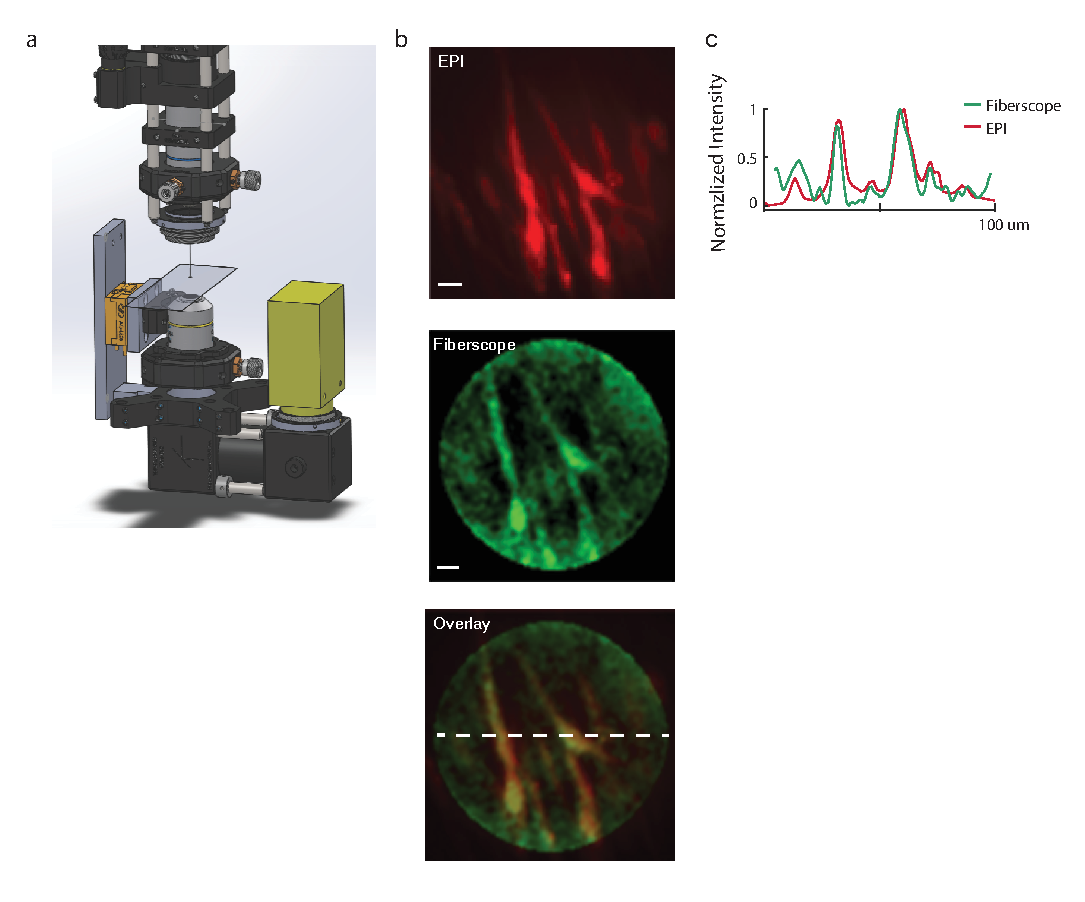
\includegraphics[width=12cm]{figure10}
\caption{\textbf{Static In-vitro Imaging}. a) Schematics of experimental setup. A glass side mounted with a sample was placed between the fiber microendoscope (top) and an epi-fluorescence microscope (bottom), where the latter served as ground truth. b) Imaging of baby hamster kidney cells expression eGFP. c) Intensity cross section of the overlay image. }
\label{fig:figure10}
\end{figure}

Next, we attempted to image dynamic samples (i.e., neuronal activity) by imaging a thin hippocampal neuronal tissue culture
expressing GCaMP6f \cite{Chen2013-qr}. We recorded full frame (100x100 $\mu m$ at a rate of $\sim$7-15Hz by sub-sampling (every other pixel) and increasing the diameter of the PSF to $\sim$2$\mu m$. Multiple neurons were observed within the FOV (figure \ref{fig:figure11}a). Spontaneous activity was observed across the population (figure  \ref{fig:figure11}b). The fluorescence time course measured with
the fiber was in good agreement with epi microscope
measurements (mean correlation : 0.54, n=6\footnote{The somewhat noisy measurements obtained with the fiber micro-endoscope were later traced to noisy originating from one of the micro-controller controlling the PMT }). 

\begin{figure}
\centering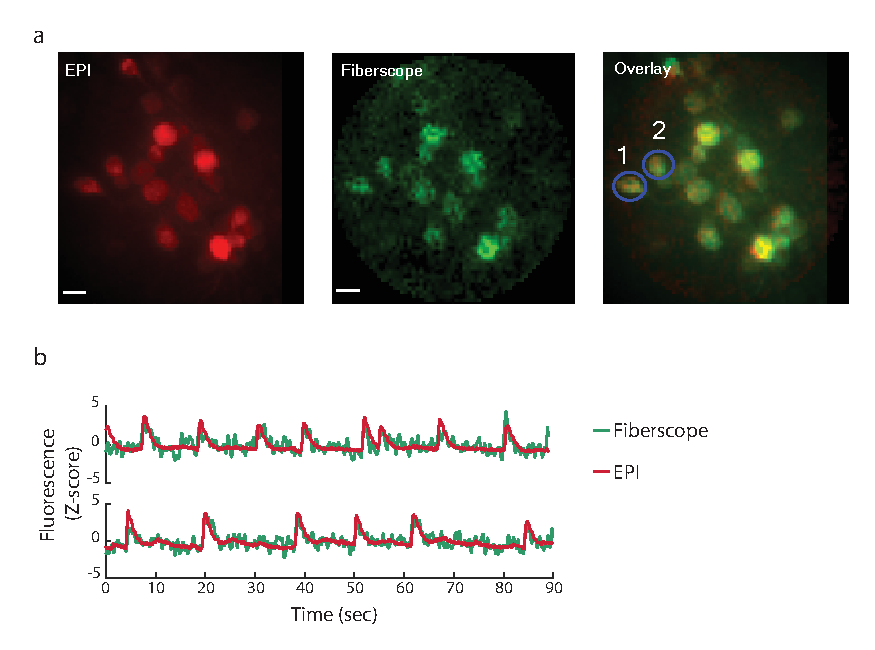
\includegraphics[width=12cm]{figure11}
\caption{\textbf{Dynamic In-vitro imaging}. a) A similar experimental setup to the one shown in \ref{fig:figure10}a was used to image hippocampal neuronal
tissue culture expressing GCaMP6f. b) Time profile of two cells (highlighted in (a)). }
\label{fig:figure11}
\end{figure}

Finally, we tested whether our system can be used to image neuronal activity in-vivo. We targeted primary visual cortex in wild-type mice that went through viral injection of GCaMP. We slowly inserted the fiber to the brain in steps of $\sim$50$\mu m$. Upon fiber insertion, several neurons appeared in the field of view (figure
\ref{fig:figure10}a) and drifted outward (towards the periphery) as the fiber was pushed in (see supplementary video). To validate that neurons were still active we calculated the standard deviation
over time (figure \ref{fig:figure10}b). Activity was strongly localized to active neurons compared to background  (see background subtracted temporal traces in figure \ref{fig:figure10}c). 

\begin{figure}
\centering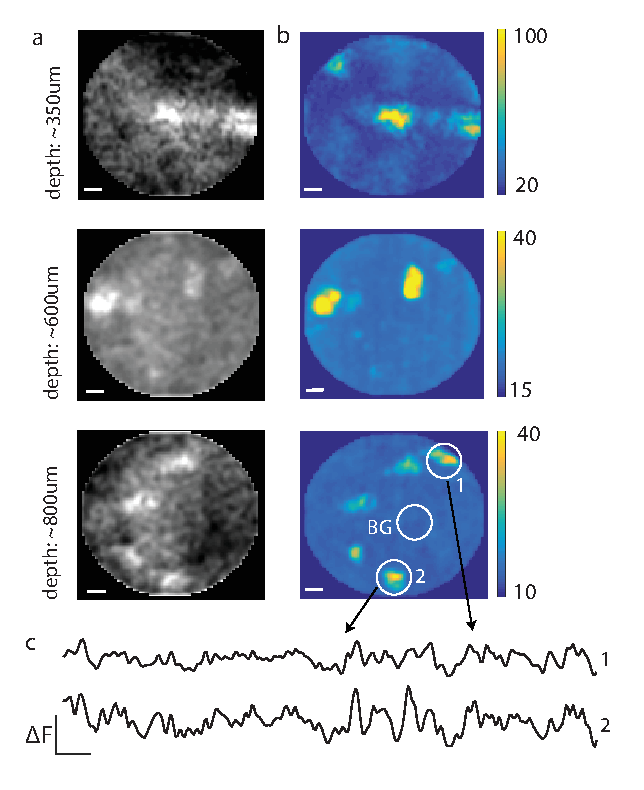
\includegraphics[width=12cm]{figure12}
\caption{\textbf{Dynamic in-vivo imaging}.
a) Imaging in-vivo neurons expressing GCaMP6f. Imaging plane was fixed at $\sim$100$\mu m$ away from the fiber tip. The fiber was inserted slowly into the tissue and videos were acquired at multiple depths. Images show the average intensity over time. b) Same location as (a), but showing standard deviation over time, which correlated directly with the amount of neural activity observed. c) Temporal traces from two example neurons after background subtraction.  
}
\label{fig:figure12}
\end{figure}

\subsection{Nuisance Factors }\label{nuisance}
A key assumption we've made so far is that the TM remains fixed throughout an experiment. However, several factors can change the transmission matrix. First, any fiber deformation is likely to change the scrambling and destroy the ability to form spots.

To address this concern we experimented with bending a long fiber in the middle while monitoring the images of fluorescent micro-spheres beneath the tip. We found that slight perturbation of the fiber position does not abruptly destroy the ability to form spots, but instead the effect is gradual and slowly degrades the SNR.  This can be nicely visualized in figure \ref{fig:figure9}a, where beads can be  easily recognized even after the fiber was shifted by 500 $\mu m$. To precisely quantify this we used the separability index  d' (\ref{fig:figure9}b), which indicated that even at displacement of 500 $\mu m$, one can still detect an object relative to the noisy background. Obviously, one would like to allow larger tolerances on fiber bending and one way forward is to engineer fibers with custom refractive profiles that may be less susceptible for such deformation (see \cite{Caravaca-Aguirre2017-wq}).

\begin{figure}
\centering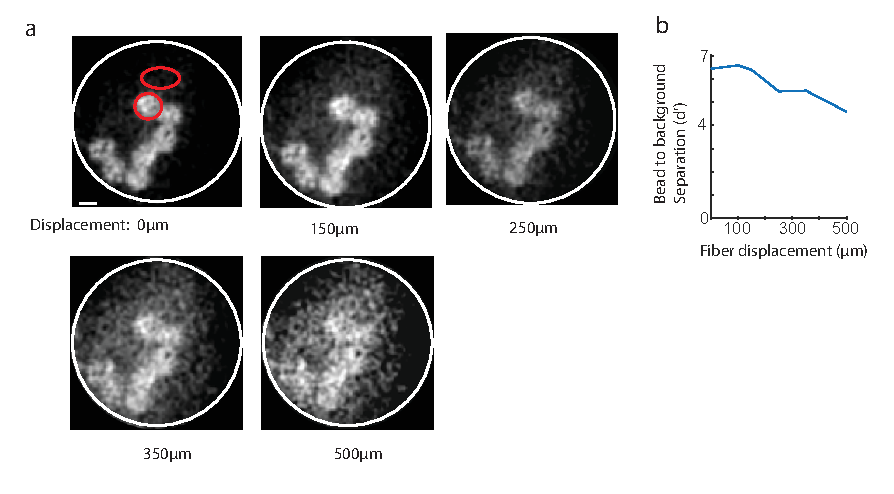
\includegraphics[width=12cm]{figure9}
\caption{\textbf{Gradual image deterioration after fiber bending}.
a) fluorescent micro-spheres were imaged with a long fiber. The middle part of the fiber was precisely translated while images were obtained to assess maximal bending allowed. b) Quantification of foreground (micro-spheres) to background SNR using the d' measure (estimated at the two red highlighted regions in (a) ).
}
\label{fig:figure9}
\end{figure}


Another nuisance factor that can change the TM is temperature. Temperature changes can lead to different expansion of the two materials forming the core and cladding, leading to different coupling of light in the fiber. Although changes in room temperature aren't a cause for concern (and indeed, once a fiber is calibrated in room temperature, the TM is robustly maintained over hours and days), inserting a fiber into warm brain tissue can cause significant changes.

To assess the severity of such nuisance factor we calibrated a fiber in room temperature and continuously measured the EF across several formed spots while slowly increasing and recording the temperature using a sensitive temperature sensor (TMP36, Analog Devices). 
We found that temperature shifts of 20 $\deg$C caused a significant reduction in the peak intensity of the generated spots (figure \ref{fig:figure8}a, blue curve), while background intensity remained roughly the same (figure \ref{fig:figure8}a, black curve). This mapped directly to a significant reduction of EF values (almost 10x, see figure \ref{fig:figure8}b). Nevertheless, even such extreme low EF values, images of fluorescent micro-spheres could still be obtained (see small inset in figure \ref{fig:figure8}b). Thus, for in-vivo experiments it may be beneficial to calibrate the fiber at warmer temperature, or find fibers that are less susceptible for temperature changes. 

\begin{figure}
\centering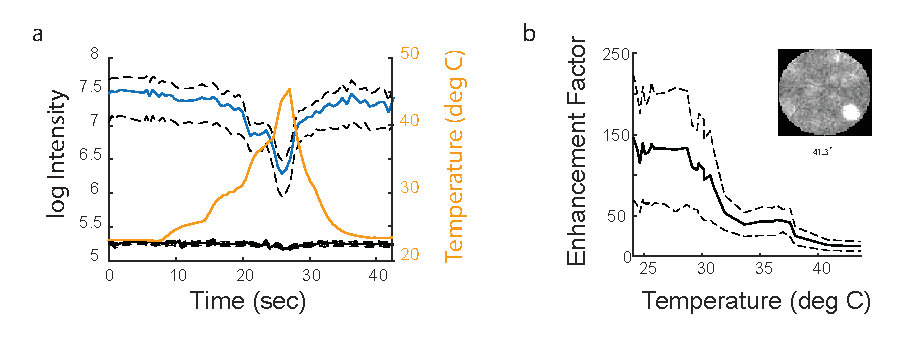
\includegraphics[width=12cm]{figure8}
\caption{\textbf{Enhancement Factor temperature fluctuations}. a) Intensity of generated point spread function at various locations as a function of fiber temperature.  Blue: peak intensity at the PSF, black: avg. intensity of background, yellow: approximated fiber temperature. b) Enhancement factor deterioration as a function of temperature. Small inset: image of a fluorescent bead taken at 41$\deg$C after a calibration at 25$\deg$C.}
\label{fig:figure8}
\end{figure}


\section{Discussion}
We present a new micro-endoscope imaging system that uses WFS on a DMD to control light in a single MMF. To the best of our knowledge, this is the first demonstration of using MMF to image live cells and in-vivo neurons and represents a significant improvement over single pixel imaging fiber photometry \cite{Gunaydin2014-ns}. The Image quality in our existing design is far from the fundamental limit and future designs will benefit greatly from improved mechanical stability (fiber coupling on the proximal side), precise temperature control, and higher EF with high-definition DMD. Nevertheless, even with the existing (non-optimal) implementation, we demonstrate it is sufficient to acquire images which allow identification of fine features at the neuronal scale. A key improvement over previously proposed methods employing LC-SLM  \cite{Barankov2014-of,Kolenderska2015-rb,Choi2012-lk,Kim2014-wo} is the ability to rapidly scan a large field of view and capture calcium events, while maintaining sufficient spatial resolution to resolve cellular details. The proposed micro-endoscope is primarily designed for head restraint animals since fiber bending of more than 1mm is likely to degrade SNR to a point where individual neurons can no longer be discriminated from the background. However, preliminary results from testing various fibers types \cite{Caravaca-Aguirre2017-wq} suggests fiber engineering is likely to reduce motion sensitivity, increase SNR and may lead to solutions that can be used for freely behaving preparations. The proposed fiber-scope addresses critical needs for deep minimally-invasive brain functional imaging: small cross-section, micron-scale resolution, real time capture of neuronal dynamics including random access scanning, high-collection efficiency, multi-spectral capability, and volumetric imaging. Therefore, we expect this technology will open new avenues for addressing circuit level questions in deep brain regions that have thus far been unreachable with existing imaging modalities \cite{Seidemann2016-no,Li2017-jr}, especially in larger animals, such as non-human primates. 








\subsection{Supplementary material}
Videos showing the calibration process and example of neuronal imaging are available at \url{https://github.com/dicarlolab/Fiberscope}/.

\newpage

\section*{Funding}
McGovern Institute for Brain Research internal seed money.
Life Sciences Research Foundation and Howard Hughes Medical Institute.
National Institute of Health Award REY026436A.  

\section*{Acknowledgments}
We would like to thank Ian Wickersham for providing samples of BHK cells, Or Shemesh and Ed Boyden for providing the GCaMP6 neuronal tissue culture and discussions throughout the project.

\section*{Disclosures}
The authors declare that there are no conflicts of interest related to this article.


\end{document}
